% TCC — Metodologia
\section{Metodologia}\label{sec:metodologia}

Esta pesquisa é aplicada e experimental e avalia um \textit{fuzzer}
\textit{black-box} orientado por contratos OpenAPI. A investigação considera
três perguntas complementares: quais divergências técnicas são observadas em
APIs distintas, com que estabilidade os comportamentos reaparecem em campanhas
repetidas e se a priorização ajuda a organizar os achados para triagem. Neste estudo, o
sistema de inferência fuzzy (FIS) atribui uma prioridade técnica a cada
anomalia observada. A pontuação não representa explorabilidade, impacto real
nem gravidade de segurança demonstrada.

As três formulações abaixo são mantidas provisoriamente para escolher a
pergunta que melhor representa o trabalho:

\begin{enumerate}
    \item \textit{Como um pipeline black-box orientado por OpenAPI pode
    produzir evidências reprodutíveis e priorizadas para a triagem de
    divergências em APIs REST durante ciclos de integração contínua?}
    \item \textit{De que forma um fuzzer black-box orientado por OpenAPI pode
    transformar divergências observadas em evidências reproduzíveis,
    deduplicadas e priorizadas para a triagem de APIs REST em ciclos de
    integração contínua?}
    \item \textit{Quais evidências de execução, estabilidade e prioridade um
    pipeline black-box orientado por OpenAPI produz ao testar APIs REST, e
    quais condições determinam sua utilidade para triagem em ciclos de
    integração contínua?}
\end{enumerate}

Nas três versões, integração contínua delimita o contexto de uso. O trabalho
não implementa workflow, plugin, quality gate ou outra integração específica
com uma esteira.

\subsection{Desenho do Estudo e Papel das Aplicações}

VAmPI, Spring Petclinic REST, crAPI e RealWorld formaram o conjunto usado para
desenvolver e caracterizar o fuzzer. Os resultados dessas aplicações permitiram
auditar a configuração inicial do mecanismo de priorização e formular sua
revisão. O Meilisearch v1.45.1 foi executado somente depois dessa revisão, como
uma aplicação externa de confirmação, sem participar do ajuste das novas regras.

As aplicações foram executadas localmente em versões fixadas e reiniciáveis.
Contratos, imagens, configuração do fuzzer e procedimentos de inicialização
foram registrados para separar mudanças do objeto avaliado de variações do
ambiente.

A coleta final terá cinco campanhas independentes para cada aplicação. Antes de
cada campanha, a aplicação e os dados necessários serão reiniciados para que o
resultado não dependa do estado deixado pela execução anterior. As quatro APIs
usadas no desenvolvimento continuarão identificadas como conjunto de pilotos. O
Meilisearch será analisado no mesmo conjunto de campanhas, mas manterá o papel
separado de aplicação externa ao desenvolvimento do FIS.

O Meilisearch já possui cinco campanhas completas. Elas serão reaproveitadas
somente se a conferência dos manifestos (arquivos de registro da execução)
confirmar a mesma revisão do fuzzer,
contrato, configuração, procedimento de reset e conjunto de artefatos exigidos
para a coleta. Se algum desses elementos não puder ser comprovado, as
campanhas serão repetidas. A data não precisa ser igual à das demais APIs; o
que precisa ser igual é o protocolo registrado.

A repetição não existe para fazer o fuzzer sortear casos diferentes. Com o mesmo
contrato, revisão e configuração, o plano de requisições tende a ser o mesmo.
Ela verifica se as respostas, os achados e as assinaturas se mantêm depois do
reset. Essa distinção é necessária porque a execução ainda pode variar: alguns
runners geram credenciais automaticamente, e o estado da aplicação, o tempo de
resposta ou uma falha transitória podem mudar entre campanhas.

\subsection{Geração dos Testes e Níveis de Mutação}

A geração começa com um caso compatível com as informações interpretadas do
contrato. A partir dele, o motor aplica operadores tipados sobre parâmetros e
corpos. Três níveis organizam a exploração:

\begin{itemize}
    \item \textbf{Nível 0 (L0) --- caso-base:} executa a entrada gerada para
    satisfazer o contrato e estabelece a referência nominal da operação;
    \item \textbf{Nível 1 (L1) --- mutação isolada:} aplica uma alteração por
    caso, permitindo relacionar a resposta com um operador específico;
    \item \textbf{Nível 2 (L2) --- mutações combinadas:} combina duas alterações
    compatíveis para explorar interações, preservando orçamento próprio e os
    casos isolados de L1.
\end{itemize}

Essa progressão distingue comportamento nominal, efeito individual e interação
entre mutações. O plano também inclui, quando habilitados, testes de operações
protegidas sem credencial ou com credencial inválida. Limites de casos,
concorrência, atraso e timeout são registrados como parte da configuração.

\subsection{Protocolo Experimental e Estratégia de Avaliação}

Cada campanha segue o fluxo contrato, plano, execução, análise e
pós-processamento. Um manifesto registra identificador do experimento, API,
repetição, revisão do código, estado Git, hashes, ambiente, configuração,
horários e contagens. O plano e os resultados são correlacionados por
\texttt{case\_id}; campanhas incompletas ou inválidas devem permanecer
identificáveis, em vez de desaparecer das evidências.

As campanhas definitivas usam a configuração já exercitada nos pilotos. O
runner percorre todas as operações suportadas pelo módulo que interpreta o
contrato e executa os níveis L0, L1 e L2. O limite configurado é de 20 casos de
mutação isolada por payload no L1 e de 10 pares compatíveis no L2. Esses limites
são fixos; a quantidade efetiva pode ser menor quando o contrato oferece menos
parâmetros, esquemas ou combinações aplicáveis. A concorrência fica em 1, o
intervalo entre requisições em 250 ms e o timeout em 10 s. A autenticação
automática é usada somente nos alvos em que o runner consegue configurá-la de
forma reproduzível.

Aqui, contrato significa o arquivo OpenAPI de cada alvo. Ele descreve as
operações, caminhos, parâmetros, corpos e respostas que o runner consegue
interpretar. Por isso, contratos diferentes geram quantidades diferentes de
casos e de requisições; não se espera que todas as APIs produzam o mesmo total.
Cada manifesto registra o número planejado e o número executado, além da
configuração usada, para que a comparação aplique a mesma regra a contratos de
tamanhos distintos.

Antes da execução, o healthcheck do alvo precisa passar. Durante a campanha,
``acessível'' significa que o processo continua disponível o suficiente para o
runner concluir o plano. Uma resposta 4xx ou 5xx de uma operação é uma
observação do teste e não invalida, por si só, a campanha. Já falha de
inicialização, falha no reset, encerramento do processo ou interrupção que deixe
requisições sem resultado impedem a interpretação completa da execução.

Uma campanha válida tem o plano completo, um resultado relacionável a cada
\texttt{case\_id}, artefatos legíveis e registro da versão do alvo, da revisão do
fuzzer e da configuração. Quando isso não ocorre, a campanha recebe status
inválido e a justificativa fica junto dos seus logs e artefatos; ela não entra no
agregado válido e não é apagada. Se a causa puder ser corrigida, uma nova
campanha é executada com o mesmo protocolo. A execução original continua
preservada como evidência da falha, e a nova execução recebe seu próprio
identificador.

\begin{figure}[H]
    \centering
    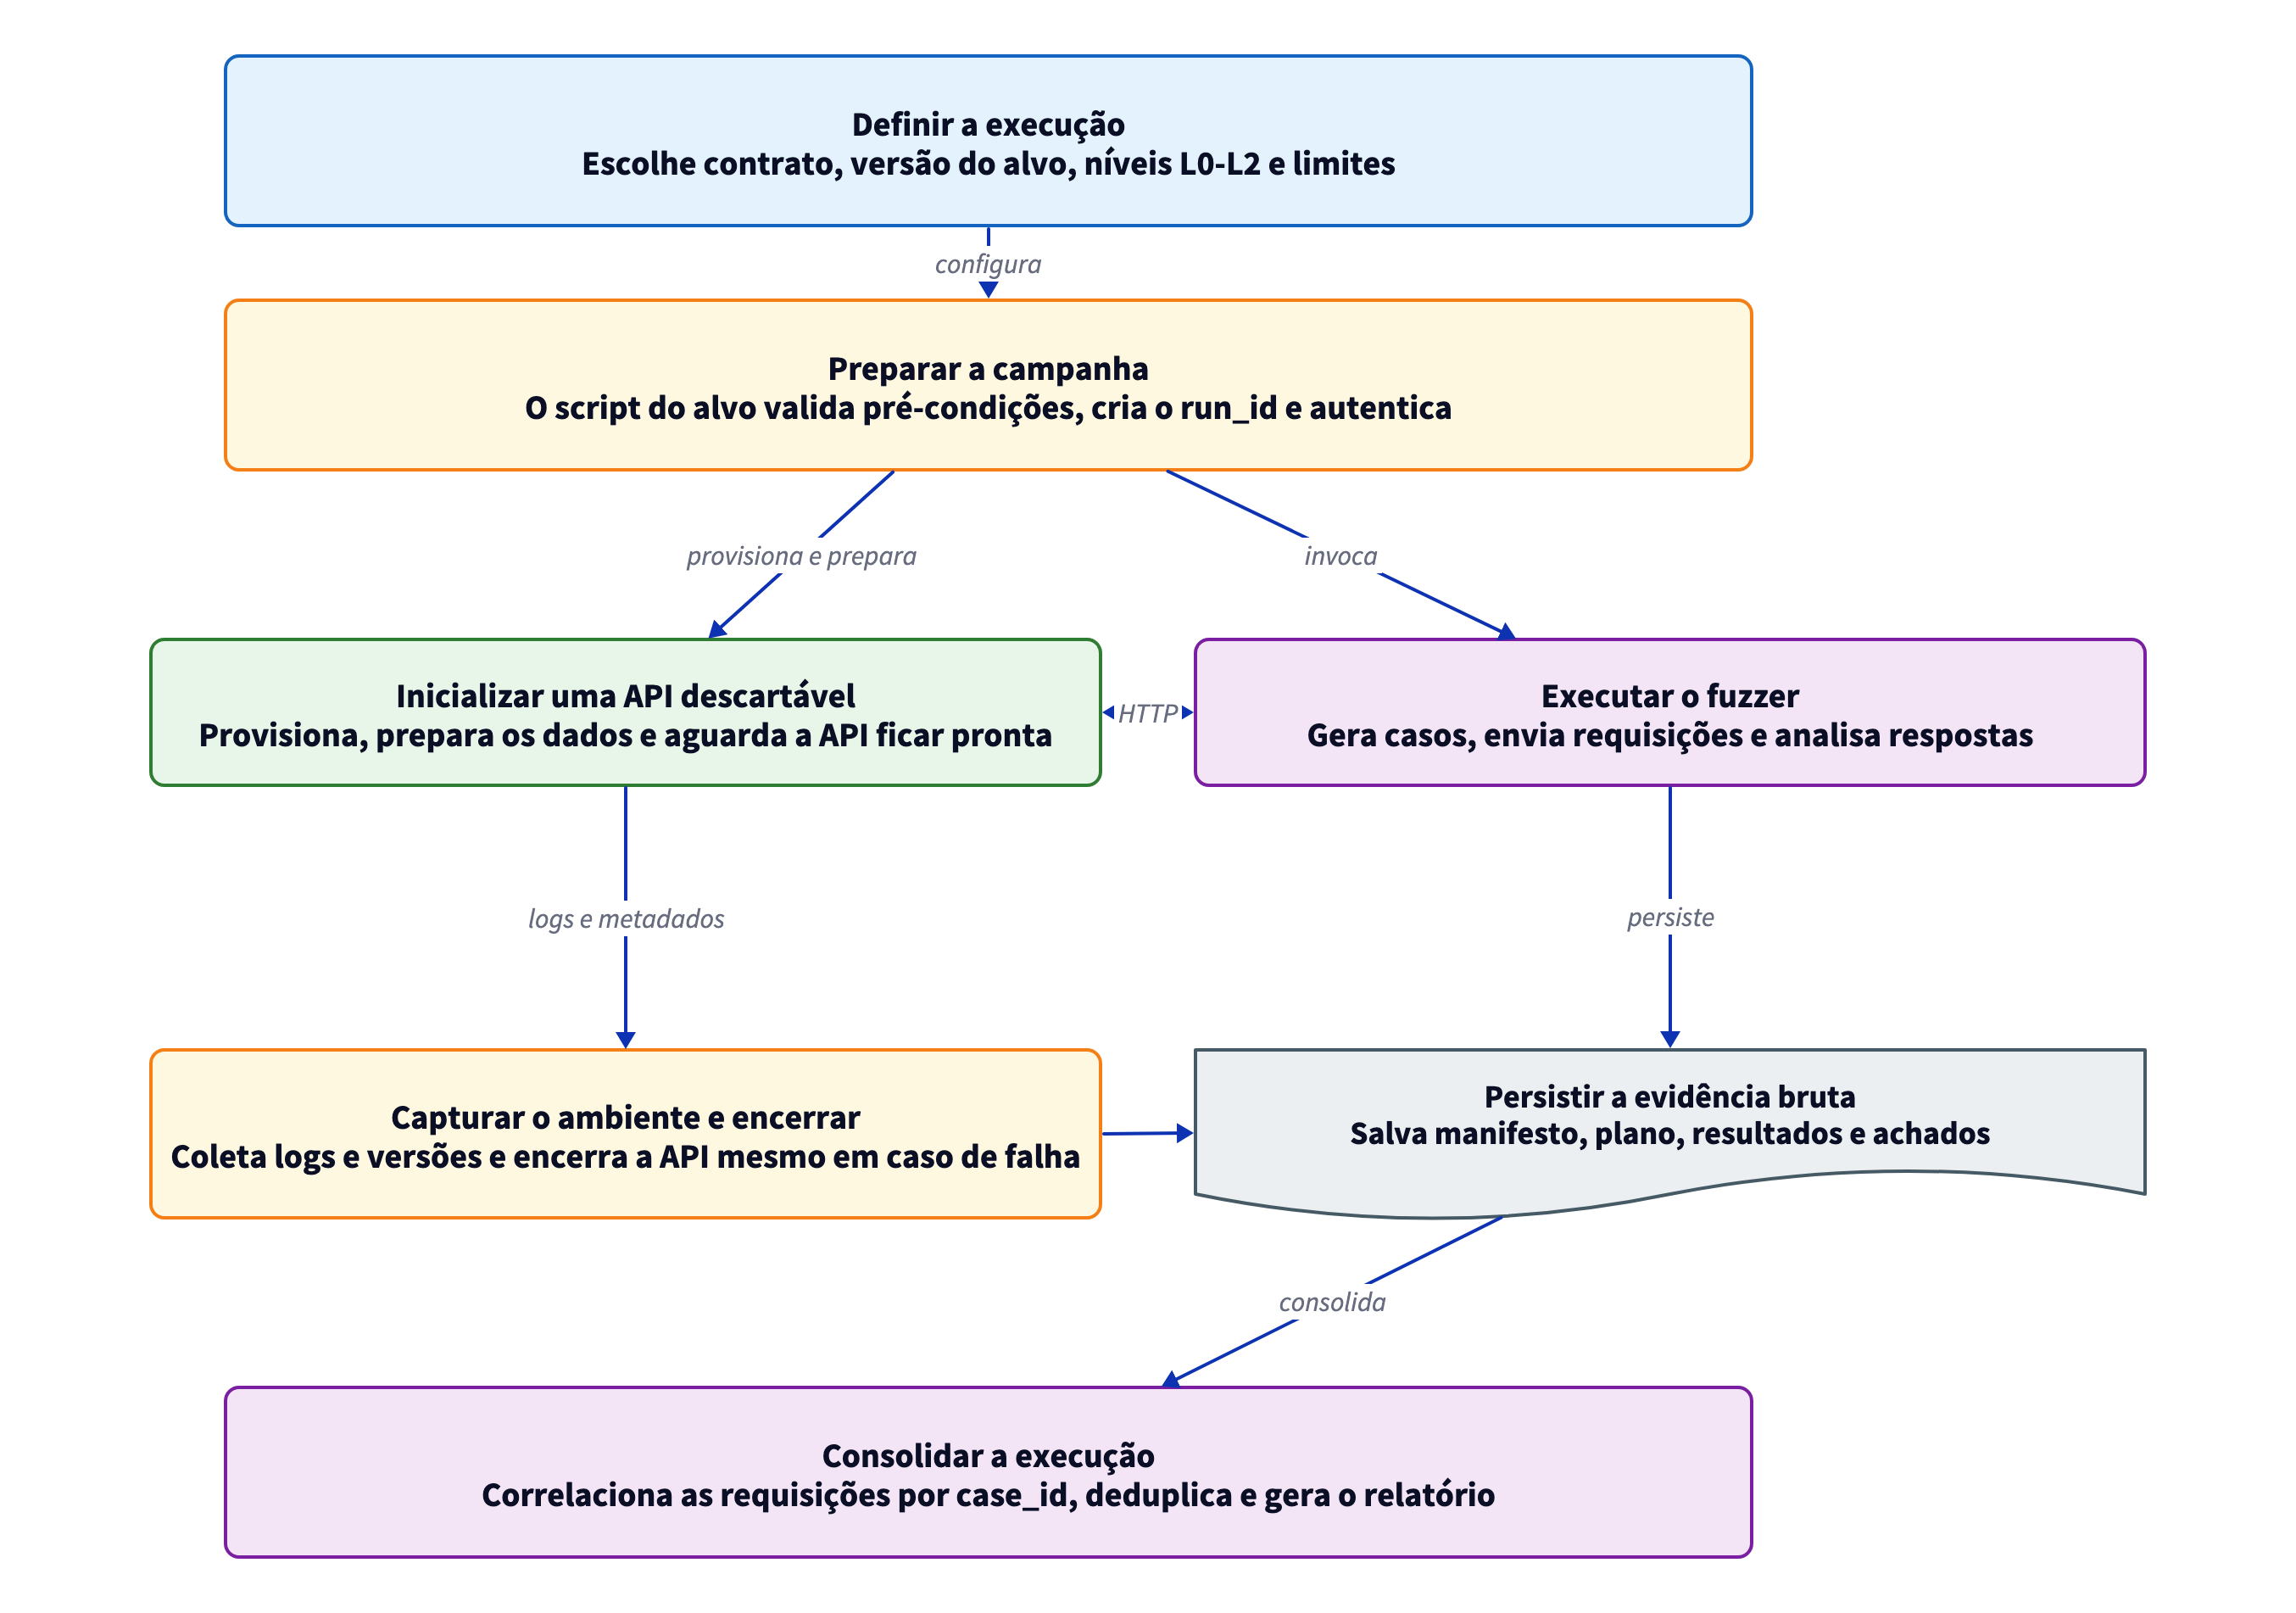
\includegraphics[width=0.90\linewidth]{Diagrams/experimental-architecture.png}
    \caption{Ciclo de uma execução experimental isolada. O script específico
    prepara o alvo descartável e invoca o fuzzer. A ligação HTTP representa a
    troca de requisições e respostas; a evidência é completada com a
    proveniência do alvo antes da deduplicação e consolidação.}
    \label{fig:ciclo-experimental}
\end{figure}

Para acompanhar uma execução sem misturar coisas diferentes, o estudo separa
cinco unidades:

\begin{itemize}
    \item uma \textbf{requisição}, que é um caso enviado à API;
    \item um \textbf{achado}, que é a divergência observada nessa requisição;
    \item uma \textbf{assinatura}, isto é, um identificador que agrupa
    observações equivalentes por aplicação, operação, classificação, status e
    resposta normalizada;
    \item uma \textbf{campanha}, que é uma execução completa contra uma API;
    \item uma \textbf{família de comportamento}, que reúne assinaturas que
    descrevem o mesmo comportamento factual por endpoint e tipo de divergência.
\end{itemize}

Essa separação evita contar várias mutações que produziram a mesma resposta
como falhas diferentes. Ela também não afirma que cada grupo corresponde a uma
causa raiz no código da aplicação.

Para comparar a prioridade atribuída pelo FIS, foi construída uma referência
independente do seu resultado. Cada família foi apresentada com o contrato, a
requisição, a resposta e a repetição observada, mas sem mostrar a classificação
do analisador nem a prioridade calculada pelo FIS. Três avaliações independentes
aplicaram a mesma rubrica de LOW, MEDIUM e HIGH. Quando não houve maioria, uma
quarta avaliação decidiu o caso sem acesso às avaliações anteriores ou ao FIS.
Essa referência serve para a comparação operacional; não é uma avaliação de
especialistas humanos e não confirma vulnerabilidades.

O FIS é comparado com uma regra mais simples, que usa apenas o desvio do status
HTTP. As duas abordagens recebem as mesmas famílias como entrada. A análise
registra a proporção de classificações iguais, o desempenho por classe (LOW,
MEDIUM e HIGH), a distância entre erros de prioridade e a correlação entre o
ranking produzido e a referência. A estabilidade é medida pela presença de
uma mesma assinatura nas cinco campanhas, sem um replay adicional de cada
requisição. Uma assinatura é considerada estável quando aparece em pelo menos
quatro campanhas sob a mesma configuração.

\subsection{Limitações e Ameaças à Interpretação}

As limitações abaixo explicam o que pode influenciar os resultados e até onde
eles podem ser generalizados.

\paragraph{O que é medido.}
O contrato OpenAPI funciona como uma referência parcial: ele descreve o
comportamento esperado, mas pode omitir regras existentes na implementação. O
fuzzer também interpreta apenas o subconjunto de OpenAPI que suporta. Por isso,
uma divergência encontrada é um comportamento que merece inspeção, não uma
prova automática de defeito ou vulnerabilidade. O FIS ordena a prioridade
técnica desse comportamento; sua pontuação não estima impacto real, explorabilidade
ou gravidade de segurança. A assinatura agrupa respostas equivalentes, mas não
identifica a causa no código.

\paragraph{Condições da execução.}
Estado residual, ordem das requisições, latência da máquina e falhas internas da
aplicação podem mudar o resultado de uma campanha. O reset entre campanhas,
concorrência 1, atraso fixo e manifestos reduzem essas diferenças. Ainda assim,
não é possível garantir que toda variação do ambiente tenha sido eliminada.

\paragraph{Alcance das aplicações.}
O estudo usa cinco aplicações: quatro participaram do desenvolvimento e dos
pilotos, e o Meilisearch foi mantido como aplicação externa para confirmar a
priorização. Esse desenho permite testar o modelo fora do conjunto de
desenvolvimento que o originou,
mas não representa a variedade de todas as APIs REST. As conclusões ficam
limitadas às aplicações, contratos, versões e configurações avaliados.

\paragraph{Força das conclusões.}
O número de famílias e a distribuição entre LOW, MEDIUM e HIGH limitam algumas
métricas. A referência de prioridade foi produzida às cegas segundo uma rubrica,
com avaliações independentes, mas não por especialistas humanos. O trabalho
também não mede cobertura de código, não implementa integração com CI ou
quality gate e não confirma vulnerabilidades automaticamente. Essas questões
ficam fora do que os resultados podem afirmar.
